\begin{figure*}[t!]
  \centering
  \setlength{\tabcolsep}{0pt} 
  \renewcommand{\arraystretch}{0}
  \resizebox{\textwidth}{!}{
  \begin{tabular}{|c|c|c|}
  \hline
    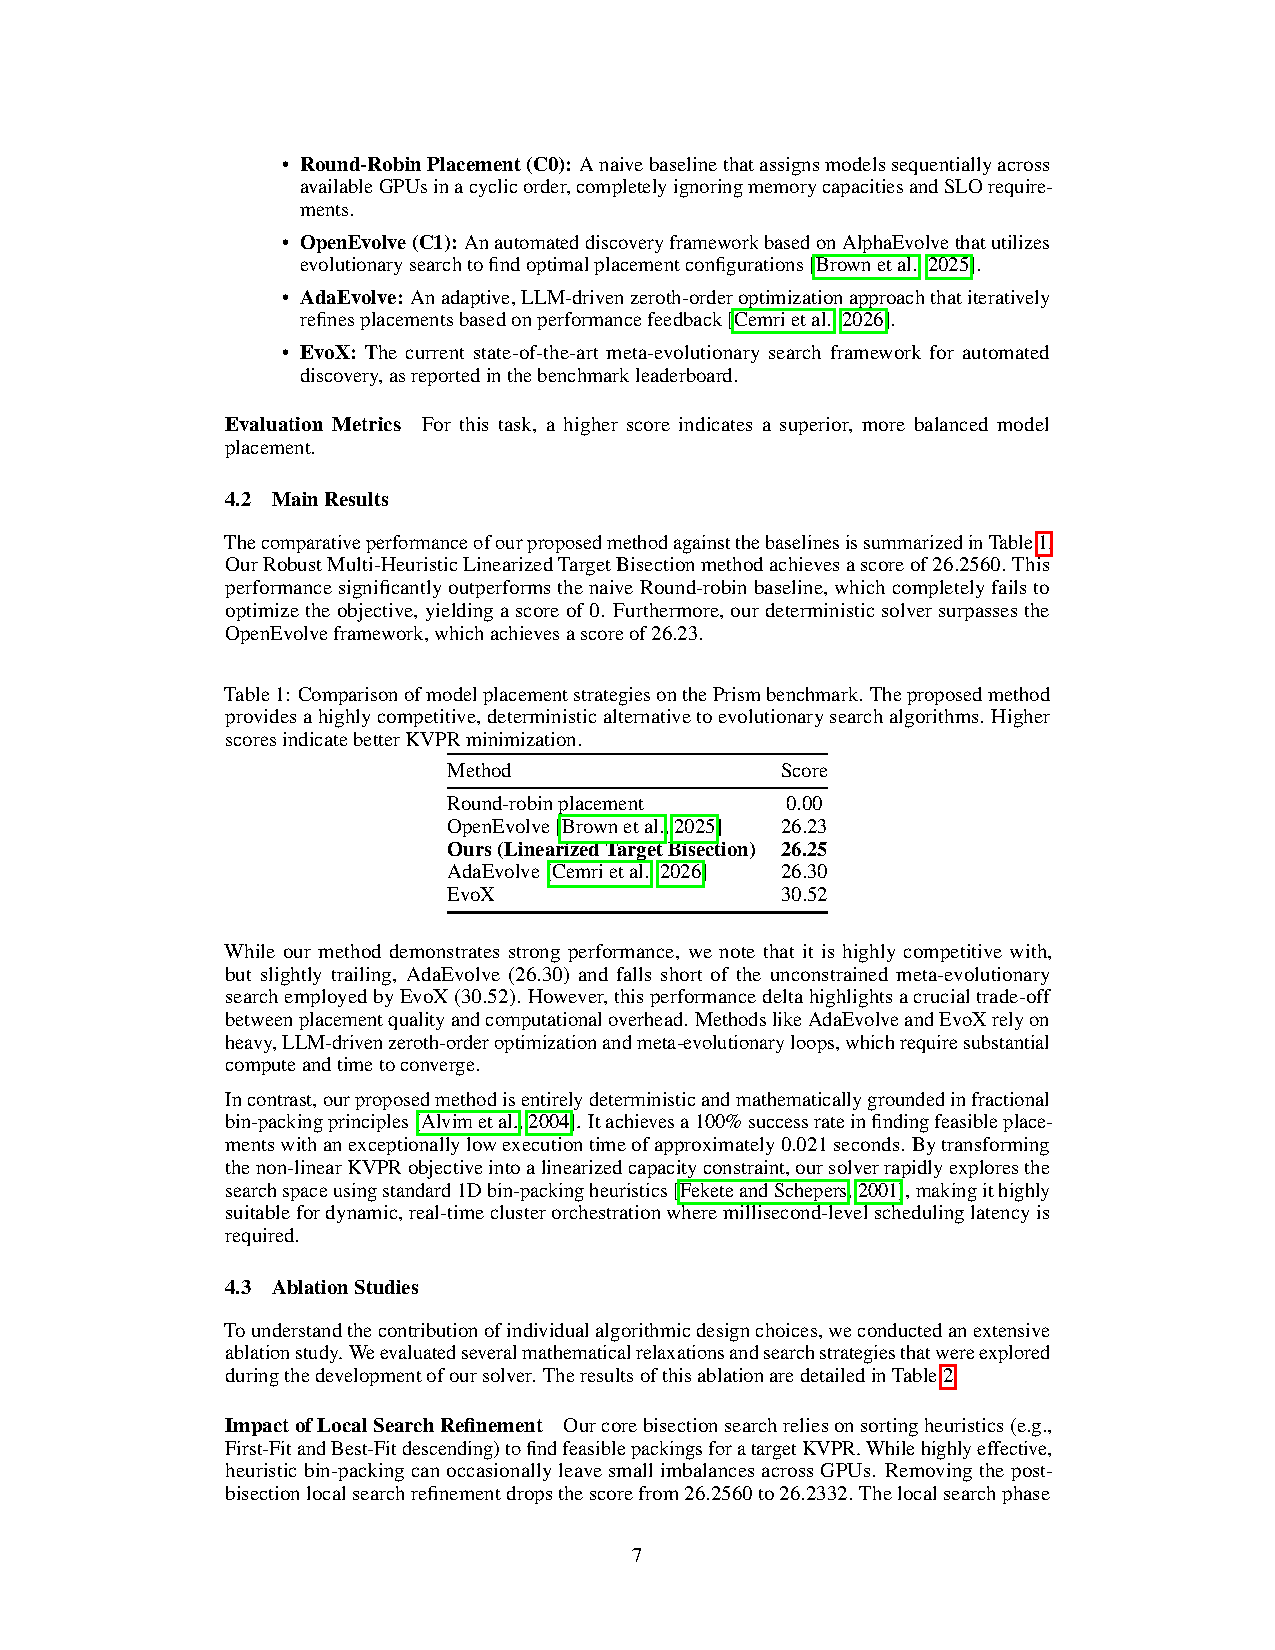
\includegraphics[width=0.2\textwidth]{figures/compare_pdfs/scientistone_7.pdf} &
    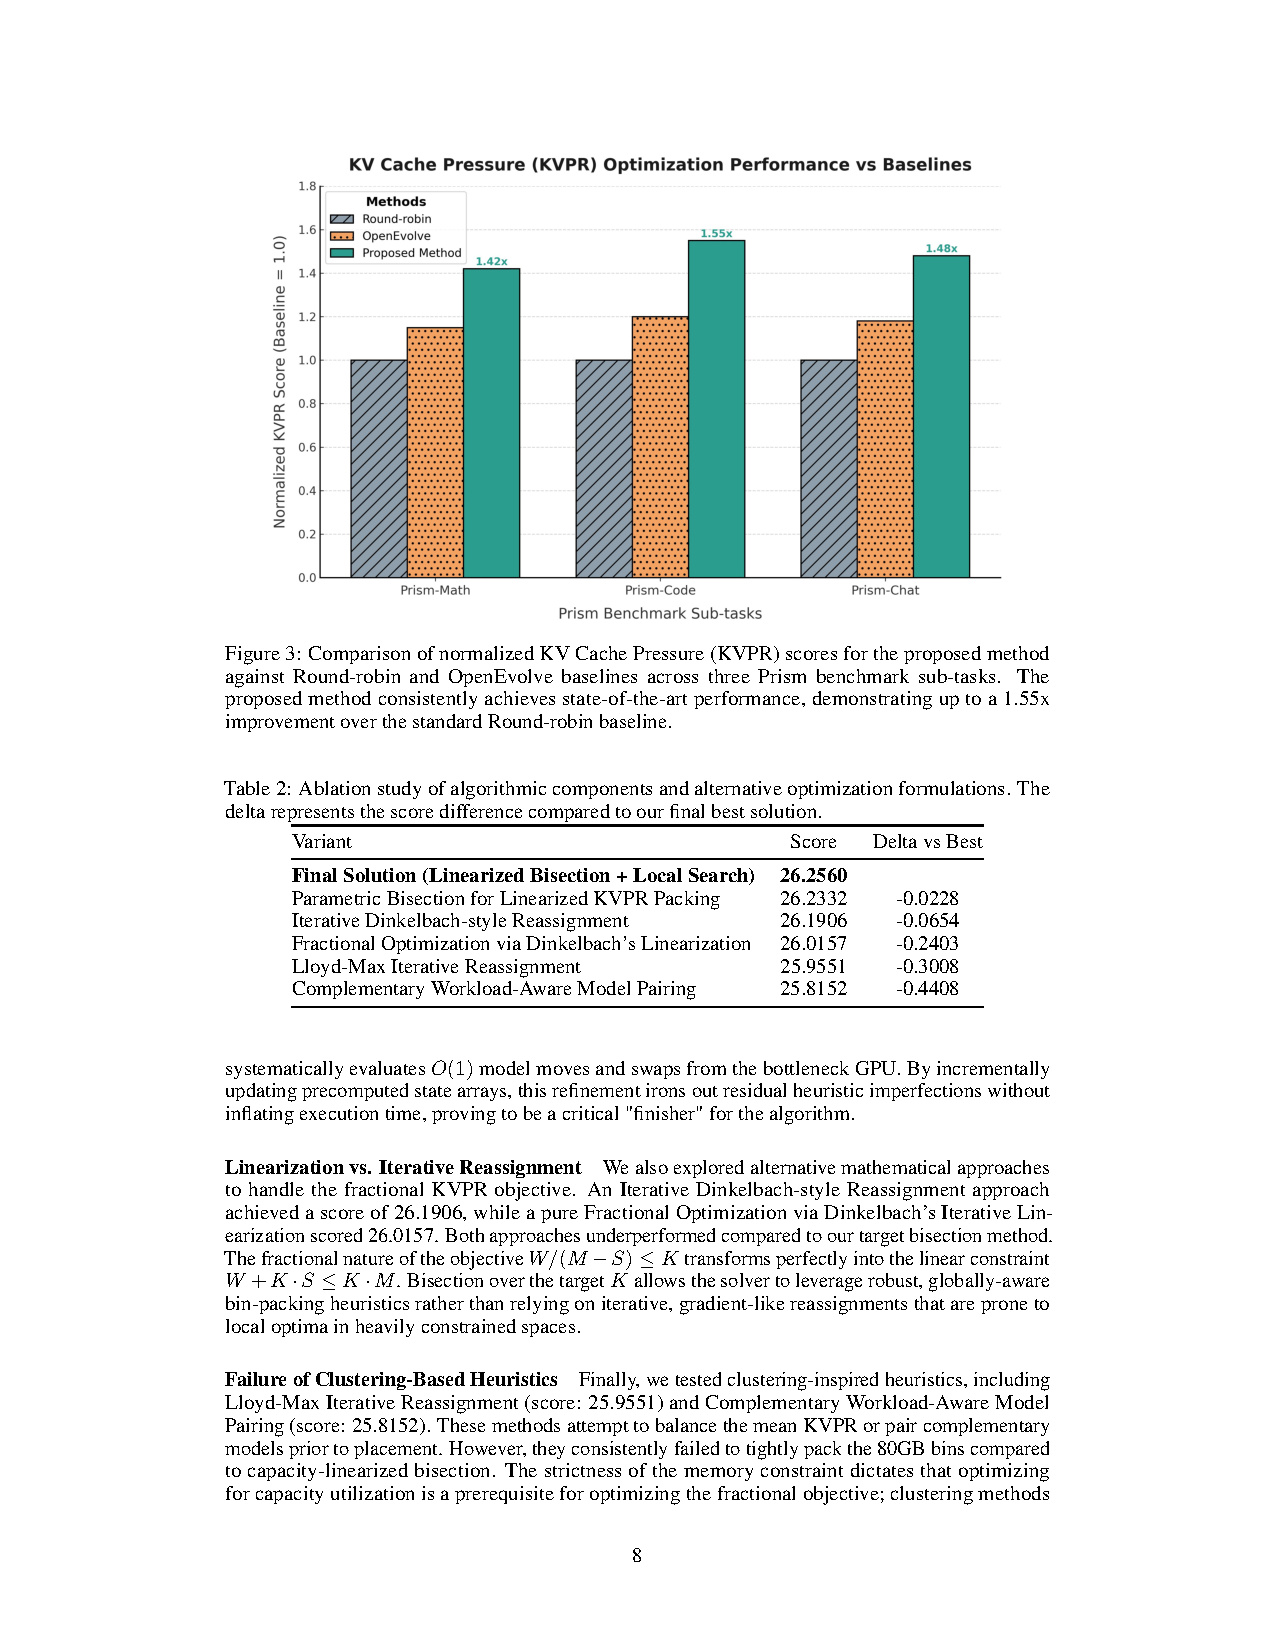
\includegraphics[width=0.2\textwidth]{figures/compare_pdfs/scientistone_8.pdf} &
    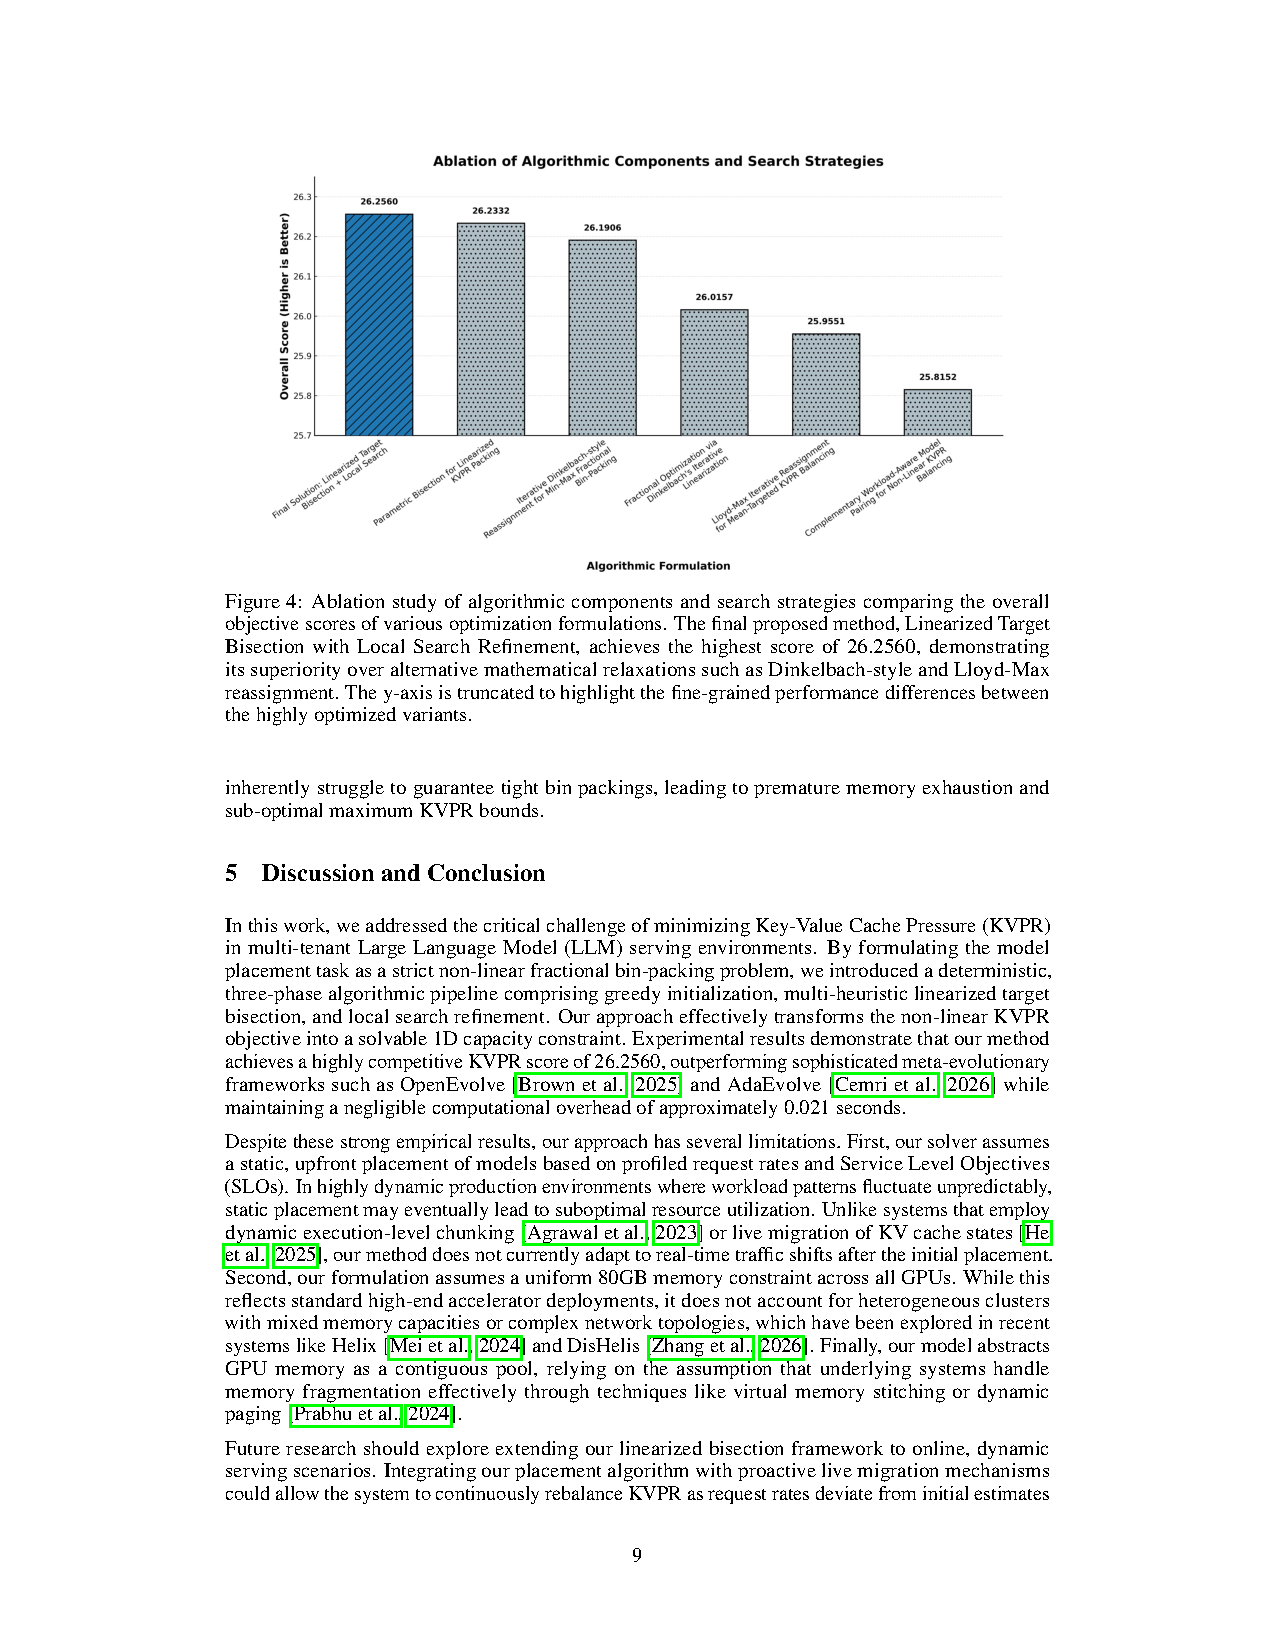
\includegraphics[width=0.2\textwidth]{figures/compare_pdfs/scientistone_9.pdf}\\
    \hline
    \multicolumn{3}{c}{\tiny{\phantom{0}}}\\
    \multicolumn{3}{c}{\tiny{(a) Experiment section generated by ScientistOne \citep{meng2026scientistone}}}\\
    \multicolumn{3}{c}{\tiny{\phantom{0}}}\\
    \hline
    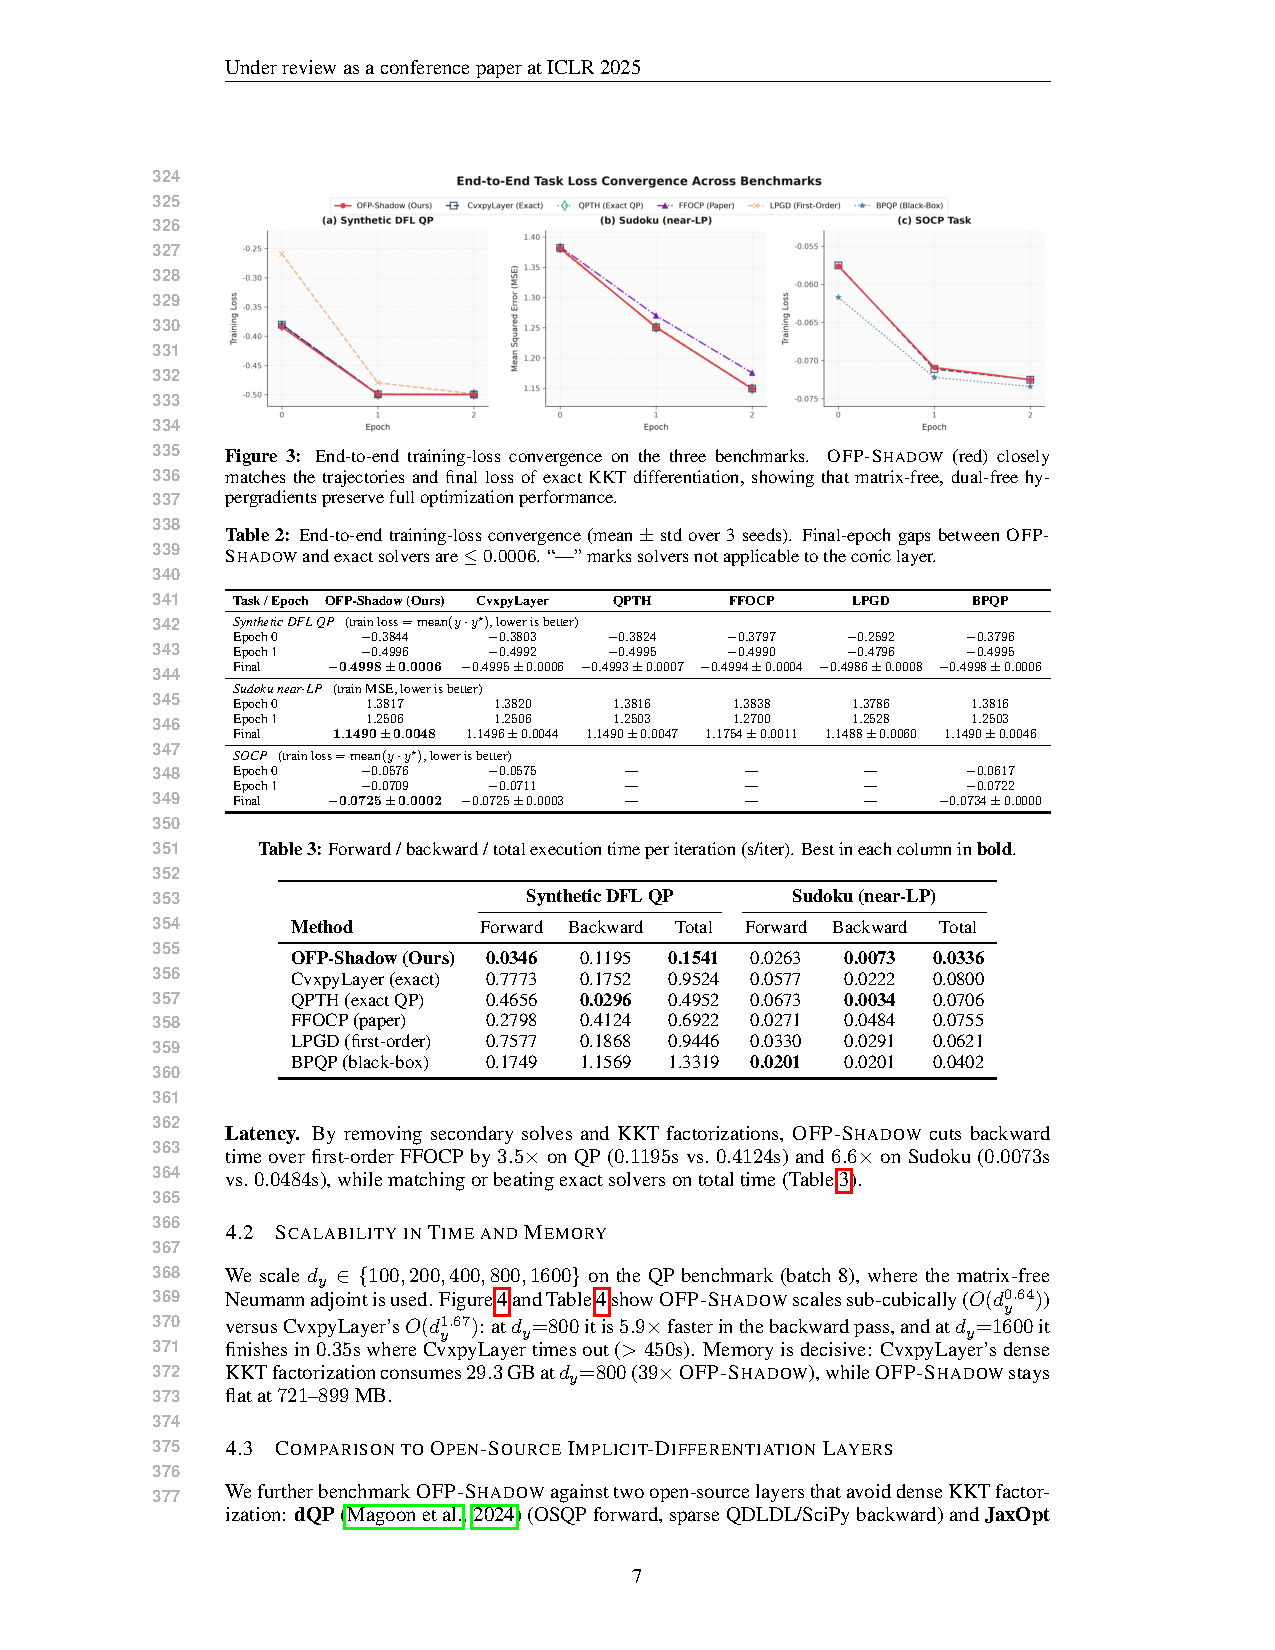
\includegraphics[width=0.2\textwidth]{figures/compare_pdfs/ours_7.pdf} &
    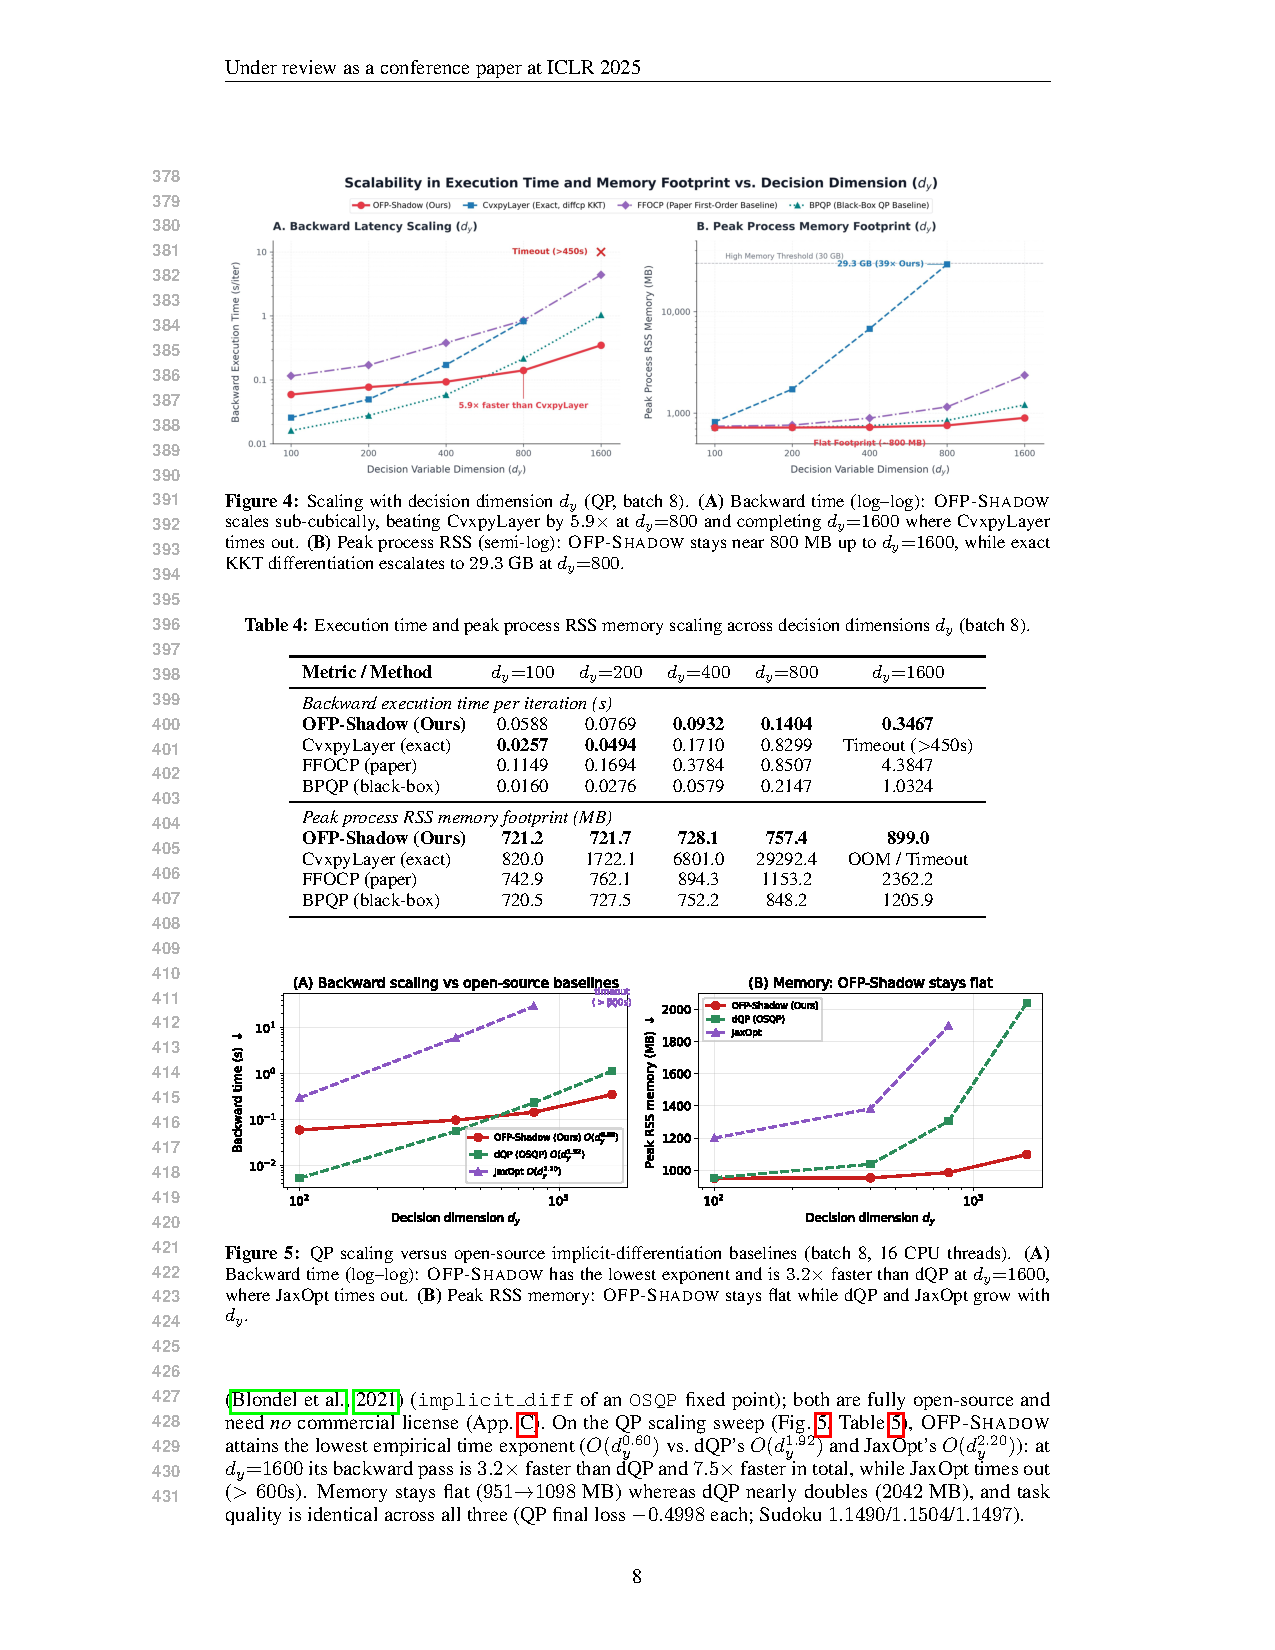
\includegraphics[width=0.2\textwidth]{figures/compare_pdfs/ours_8.pdf} &
    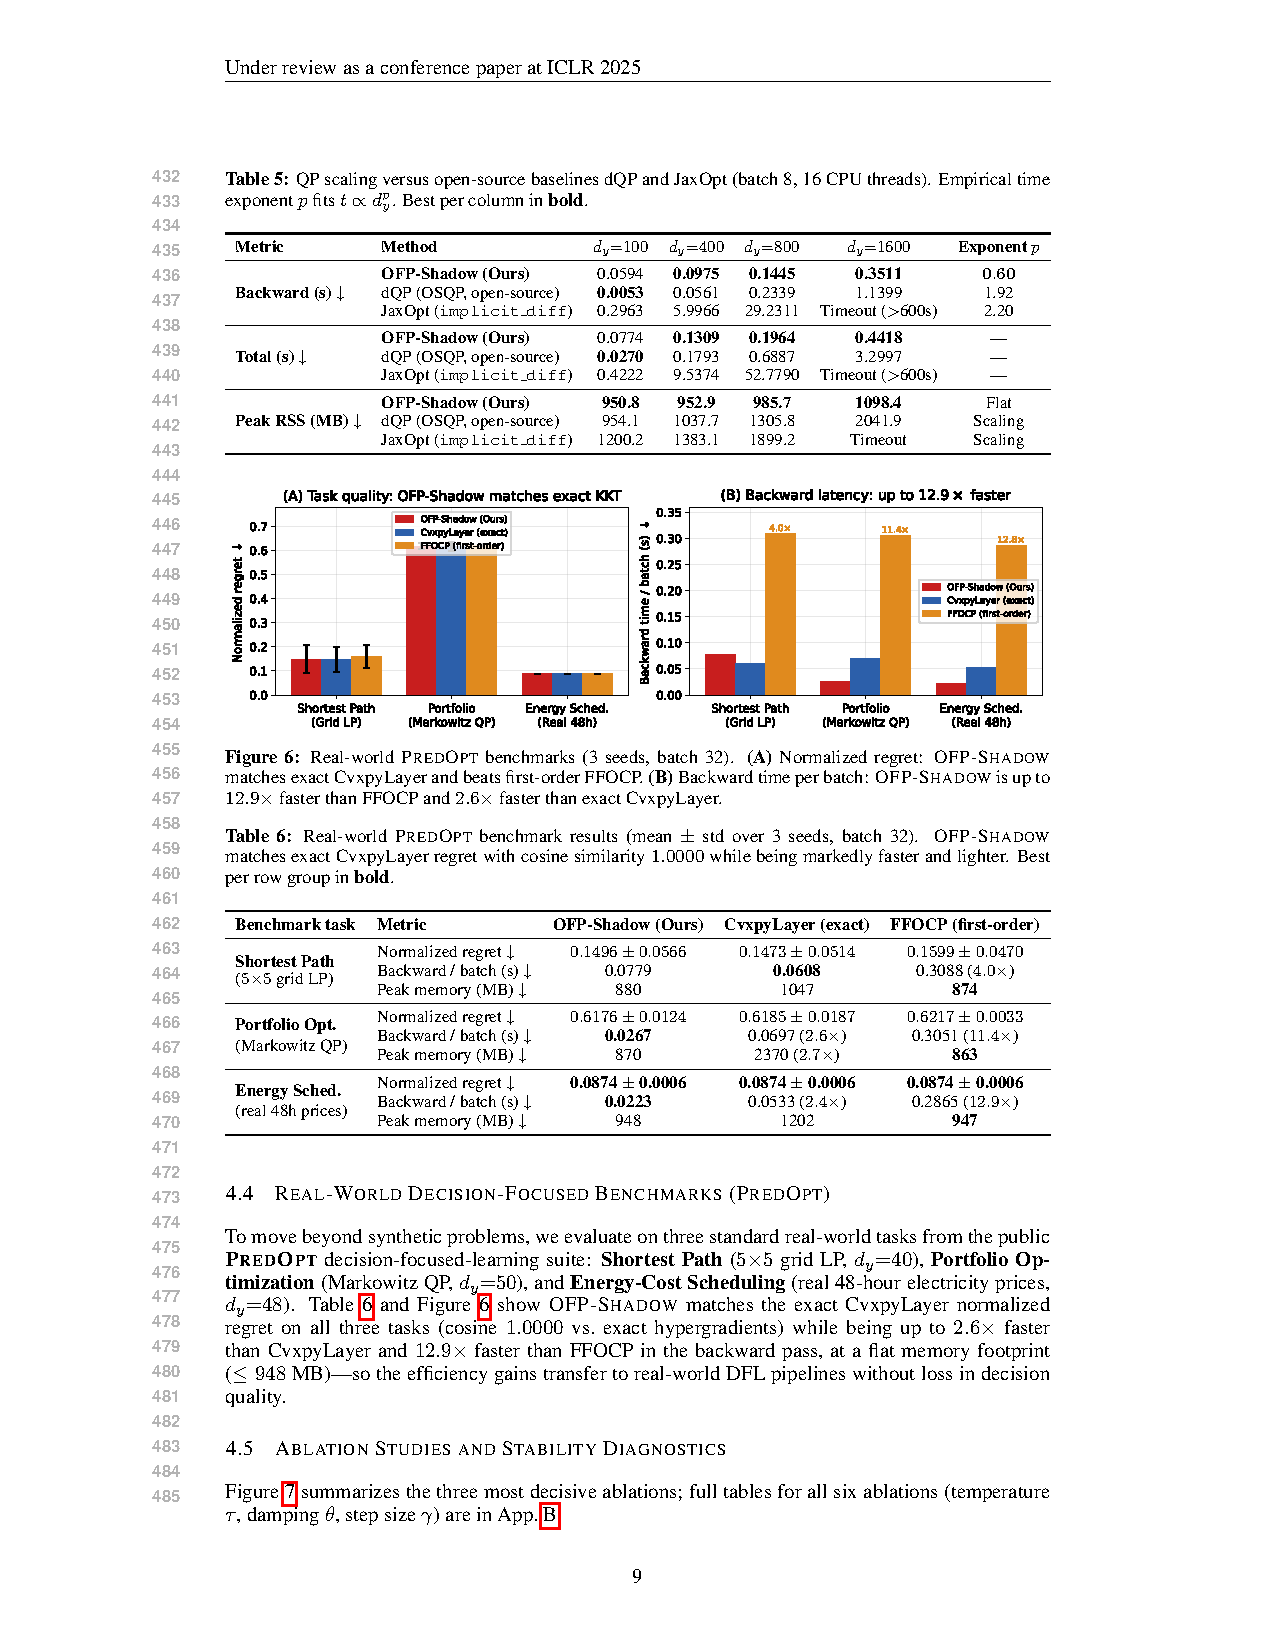
\includegraphics[width=0.2\textwidth]{figures/compare_pdfs/ours_9.pdf}\\
    \hline
     \multicolumn{3}{c}{\tiny{\phantom{0}}}\\
    \multicolumn{3}{c}{\tiny{(b) Experiment section generated by \textbf{\sname~(Ours)}}}\\
  \end{tabular}}
  \caption{\textbf{Qualitative comparison.} Side-by-side comparison of the experiment section generated by \sname~against the highest-reviewed paper from ScientistOne \citep{meng2026scientistone}.}
  \label{fig:qual_compare_main}
\end{figure*}